\section{The Mankiw-Shapiro and Stambaugh bias.}


\begin{answer}[Part a]
Start from the predictive system that you estimated in the previous question for the sample from 1945-2020.
\begin{align}
r_{t+1} &= a_r + b_r pd_t + \epsilon_{t+1}^r \label{eq:3a1}\\
pd_{t+1} &= a_{pd} + \phi pd_t + \epsilon_{t+1}^{pd} \label{eq:3a2}
\end{align}
We want to simulate from this model. Assume that the errors are normally distributed. Estimate and report the coefficients, including the covariance matrix of the shocks.
\end{answer}
I demean the data so the constant terms can be ignored in the simulation. I estimate by OLS
\begin{align}
b_r &\approx -0.096 \\
\phi &\approx 0.944 \\
\text{Cov}(e_{t+1}^r , e_{t+1}^{pd} ) &\approx 0.00694 \\
\text{Var}(e_{t+1}^r) &\approx 0.0247 \\
\text{Var}(e_{t+1}^{pd}) &\approx 0.0219.
\end{align}





\begin{answer}[Part b]
Simulate 10,000 samples of 67 observations and estimate the model for each of the samples. Importantly, fix the seed for the subsequent exercises at the beginning of each of the 10,000 runs. Compute the average estimate of $b_r$ and $\phi$ and compare them to the population values.
\end{answer}
I follow the Monte Carlo simulation outlined in \cite{mankiwshapiro1986}. Let all simulated variables be denoted with a tilde on top of their data counterparts. Let $N=75$ denote the number of observations and $M=10,000$ denote the number of runs of the simulation.

In each run of the simulation, I draw $N$ observations of $\tilde{\epsilon}^r_{t+1}$ and $\tilde{\epsilon}^{pd}_{t+1}$ from a bivariate Normal distribution with mean 0, variance 1 and correlation equal to the sample correlation between $\epsilon^r_{t+1}$ and $\epsilon^r_{t+1}$. Next, we generate simulated returns and price-dividend ratio. Set $\tilde{r}_{t+1} = \tilde{\epsilon}^r_{t+1}$. $\tilde{pd}_t$ is simulated from \eqref{eq:3a2} using $\tilde{\epsilon}^{pd}_{t+1}$ and $\phi$ estimated from the data. The initial value $\tilde{pd}_0$ is drawn from a univariate Normal distribution with mean 0 and variance $1/(1-\phi^2)$. Then using the simulated data, we run the regressions \eqref{eq:3a1} and \eqref{eq:3a2}. This completes one run of the simulation. Then repeat for a total of 10,000 runs.

From the simulation I obtain $\tilde{b}_r \approx 0.0382$ with a standard deviation of 0.0456, and $\tilde{\phi} \approx 0.923$ with a standard deviation of 0.0484. The persistence of the price-dividend ratio is quite close to the data, but the return predictability coefficient is a bit off.

\pagebreak
\begin{answer}[Part c]
Now repeat the exercise but setting the covariance
\begin{align}
\text{Cov}(\epsilon_{t+1}^r , \epsilon_{t+1}^{pd} ) =0.
\end{align}
Comment on the difference.
\end{answer}
From the simulation I obtain $\tilde{b}_r \approx 0$ with a standard deviation of 0.0437, and $\tilde{\phi} \approx 0.923$ with a standard deviation of 0.0483. The persistence of the price-dividend ratio is quite close to the data, but the return predictability coefficient is now closer.

From \cite{stambaugh1999}, we know that when returns are regressed on lagged persistent variables, the disturbances are correlated with the regressor's innovation. In the case of price-dividend ratio regressions, this creates a downward bias. In part b, we allowed for covariance between the two error terms and found a much higher point estimate of the regression coefficient $\tilde{b}_r$. When we remove that covariance in part c, the bias decreases (we find a lower estimate of $\tilde{b}_r$.


\begin{answer}[Part d]
Set the covariance back to the sample estimate, but now plot the bias in $b_r$ and $\phi$ as a function of $\phi$ where we vary $\phi = \lambda \hat{\phi}$ for $\lambda = 0, 0.1, \dots, 0.9, 1$. $\hat{\phi}$ denotes the OLS estimate obtained in part 3a. Comment on the results.
\end{answer}
To make the notation a bit clearer, now I vary the value of $\phi$ (estimated from the data) that is used as an input for the Monte Carlo simulation. I use $\lambda \phi$ for $\lambda = 0, 0.1,\dots,0.9,1$. Figure \ref{fig:q3} plots the values of $b_r$ vs $\tilde{b}_r$ on the left, and $\phi$ vs $\tilde{\phi}$ on the right, both against $\lambda$. Simulated values are in blue, while red shows point estimates from the data.

When the predictor variable is less persistent, then $\tilde{\phi}$ diverges from $\phi$ mechanically. I find this plot a bit hard to read: as the true $\phi$ varies, then so would the true $b_r$. So as you vary the input $\phi$, you would also want to vary $b_r$ due the changing $\phi$. However, we have not done that (the red lines are flat). From \cite{stambaugh1999}, as the price-dividend ratio gets less persistent ($\phi$ decreases) then the bias would get closer to 0, especially when $\epsilon_{t+1}^r$ and $\epsilon_{t+1}^{pd}$ are correlated.


\begin{figure}[!h]
\caption{\textbf{Plot of Simulated vs. Estimated Parameters}} \label{fig:q3}
  \center \vspace{-4ex} 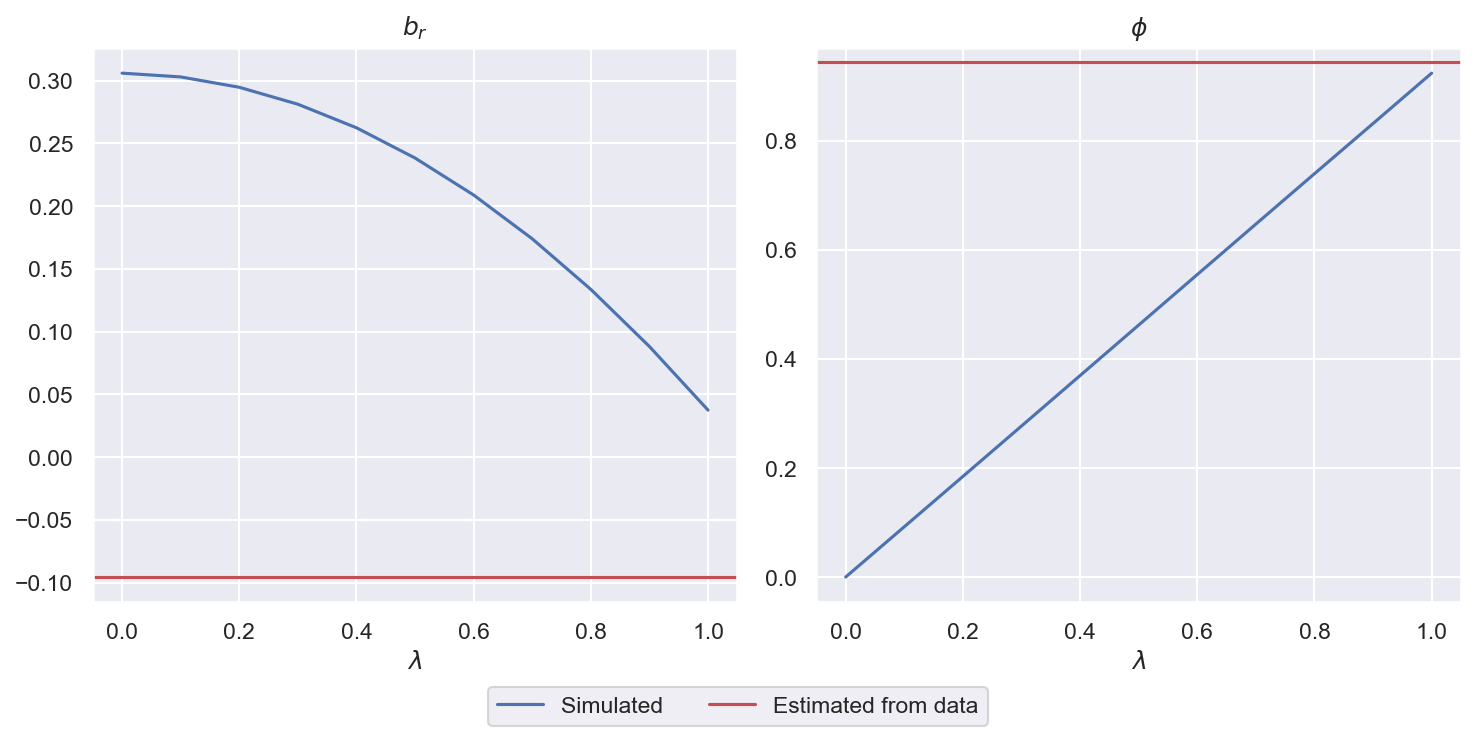
\includegraphics[width=5.5in]{../Figures/q3}		
 \begin{minipage}[c]{\textwidth}   \setstretch{1.00}
  \small \textbf{Note:} Figure shows the simulation that estimates the expected time until vaccine deployment.
 \end{minipage}
\end{figure}

